\section{eSalud}

La eSalud es definida por la organización Mundial de la Salud (OMS) \cite{oms2016} como \begin{quote}el apoyo que la utilización costo eficaz y segura de las tecnologías de la información y las comunicaciones ofrece a la salud y a los ámbitos relacionados con ella, con inclusión de los servicios de atención de salud, la vigilancia y la documentación sanitarias, así como la educación, los conocimientos y las investigaciones en materia de salud\end{quote}, en si es un término que define un campo multidisciplinar que integra componentes de diferentes áreas del saber que incluye entre otros a la medicina, la ingeniería electrónica, la telemática, la informática, la ingeniería de sistemas, la inteligencia artificial, la biónica, la psicología, la sociología, la antropología, las geociencias, entre muchas otras. Las redes eSalud consideran elementos que van mucho más alla del simple despliegue de redes tecnológicas de intercomunicación y se plantean como redes de interacción social cuyo objetivo primario - más no el único, es la prestación de servicios médicos y relacionados.

Dependiendo el grado en que se presente cada uno de los elementos mostrados en la figura ~\ref{elementosred} y de la mayor o menor correlación entre ellos, se pueden crear sistemas de eSalud que se acerquen al ideal de proveer servicios de salud de alta calidad. 


La OMS y la Unión Internacional de Telecomunicaciones (ITU) proveen \cite{ituoms2012} un método que podría ser utilizado para abordar el desarrollo de proyectos de eSalud complejos, dinámicos y evolutivos. 

\begin{figure}
 \centering
 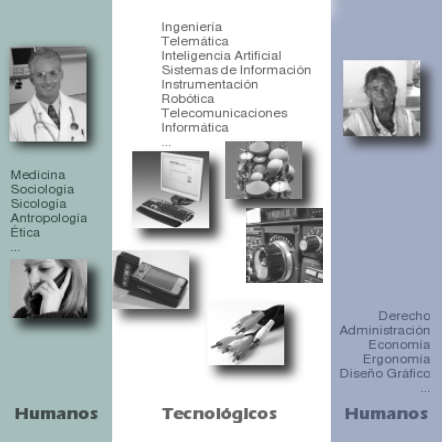
\includegraphics[width=156mm, height=156mm]{sistema_telemedicina.png}
 \caption{Elementos genéricos y áreas del saber de una red de Telemedicina}
 \label{elementosred}
\end{figure}

\subsection{Componentes Principales de eSalud}

La eSalud comprende otras áreas que, aunque no tienen una división concreta, han emergido para enfocarse en ciertos aspectos de interés:

\begin{itemize}
 \item Telemedicina: Provisión remota de servicio clínicos
 \item Telesalud: Telemedicina, complementada con la prestación remota de otros servicios tales como entrenamiento médico, monitoreo de pacientes, cuidado médico, gestión administrativa, etc. 
 \item mSalud: telesalud con el apoyo de dispositivos móviles.
 \item Registro Médico electrónico: Conocido como Historia Clínica Electrónica. Comprende los mecanismos que permiten registrar en un entorno digital seguro, la información sobre los eventos de salud de cada paciente.
 \item eAprendizaje/eEnseñanza: Servicios de enseñanza/aprendizaje de ciencias médica y afines, en modalidad a distancia o virtual.
\end{itemize}

Cabe la pena aclarar que la pluralidad de componentes no es más que un esfuerzo para abordar en un único modelo todas las tendencias que se han presentado en la evolución de la eSalud. En alguna literatura estos términos son intercambiables dependiendo el enfoque del autor. \cite{oms2010}.

\subsection{Caracterización de Capacidad para eSalud}

Diferentes organizaciones \cite{ops2011},\cite{oms2016}, \cite{ituoms2012}, han determinado que los proyectos de eSalud abarcan componentes que transcienden la parte médica y tecnológica. Consideran que aspectos de estrategia, organización, política - entre otros; son claves para el éxito de las iniciativas. En este sentido, el grupo de investigación decide desarrollar un proyecto enfocado en la caracterización multidominio de los sistemas de salud para poder determinar la capacidad que estos presentan para poder desarrollar eSalud. 

La fase actual del SITEM se centra en varios componentes: médicos, tecnológicos, administrativos, humanos y financieros. Sin embargo, debido al perfil de profesionales que han participado en el desarrollo, los elementos tecnológicos han sido mejor caracterizados hasta el momento.

\begin{figure}
 \centering
 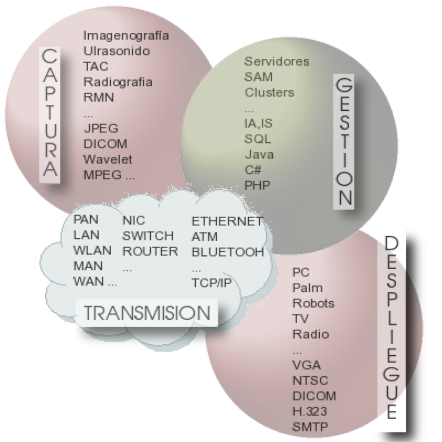
\includegraphics{red_1.png}
 \caption{Componentes en un Sistema de eSalud. Fuente: OMS/ITU}
 \label{subcomponentes}
\end{figure}

Para facilitar el análisis y modelado en la dimensión tecnológica, un sistema de eSalud - con enfoque de Telemedicina, puede reducirse a cuatro subsistemas: \cite{aparicio2003}

\begin{itemize}
 \item \textbf{Subsistema de Captura de datos:} Conformado por los dispositivos de hardware, los protocolos y aplicaciones software que trabajan conjuntamente para transformar información médica en datos susceptibles de ser administrados usando técnicas digitales.
 \item \textbf{Subsistema de Transmisión de Datos:} Hacen parte de este subsistema los dispositivos de hardware, las tecnologías de interconexión, los protocolos y aplicaciones que permiten estructurar redes de transmisión de datos digitales de una manera fiable en tiempos aceptables para un servicio específico.
 \item \textbf{Subsistema de Gestión de Información:} Dispositivos de hardware - computadores, sistemas de almacenamiento masivo, etc; y  sistemas de información que almacenan, procesan, distribuyen, analizan, integran y producen información con base en los datos de los subsistemas de captura, históricos y de pronóstico.
 \item \textbf{Subsistema de Despliegue de información:} Elementos de hardware (pantallas, transductores, sistemas de audio, etc), aplicaciones software y protocolos asociados que permiten recibir y reproducir información médica. 
\end{itemize}

Todos ellos necesariamente interrelacionados por medio de interfaces y protocolos definidos. El uso de estándares abiertos es de vital importancia para permitir que estos subsistemas puedan ser interoperables. Esto se ha logrado en gran medida en el subsistema de transmisión de datos pero aún se encuentran serios problemas en los demás, debido al sinnúmero de patentes - y protocolos propietarios, que las empresas fabricantes de dispositivos médicos aún ostentan.